\section{Bidirectional Transformation with Triple Graph Grammars}

For the third part of our tutorial, we will be introducing bidirectional transformations via triple graph grammar to our hospital example. Triple Graph Grammar (TGG) is a rule-based and declarative way to describe the language of all pairs of models that are considered to be consistent with each other. While these rules can be used to generate arbitrary consistent models from scratch, a TGG can also be used to automatically derive consistency management operations such as translators or synchronizers. In the case of our hospital, we created a metamodel view of the way the hospital might be perceived by a patient. From the viewpoint of the administration, other factors have to be considered to keep the very same hospital running, such as the salary of each staff member or their shift plans. This second administrative perspective contains new information but also information that overlaps with the patient perspective we already covered in the previous chapters and we have to make sure changing information is updated for both perspectives. For this purpose, we will be creating another metamodel from a different point of view. And throughout this chapter, we will be linking those two sides together to create our consistent triple grammar graph.

\subsection{Administration metamodel}

Let us look at the visualization of the administration metamodel in the chart below. You might notice some familiar classes like the staff and the patients, but from the administrative point of view, we want to manage our staff to cover the patients differently. Moreover, we want to keep track of the shifts a staff member covers, so every patient is cared for throughout the day.\newline 

\begin{figure}[h]
    \centering
    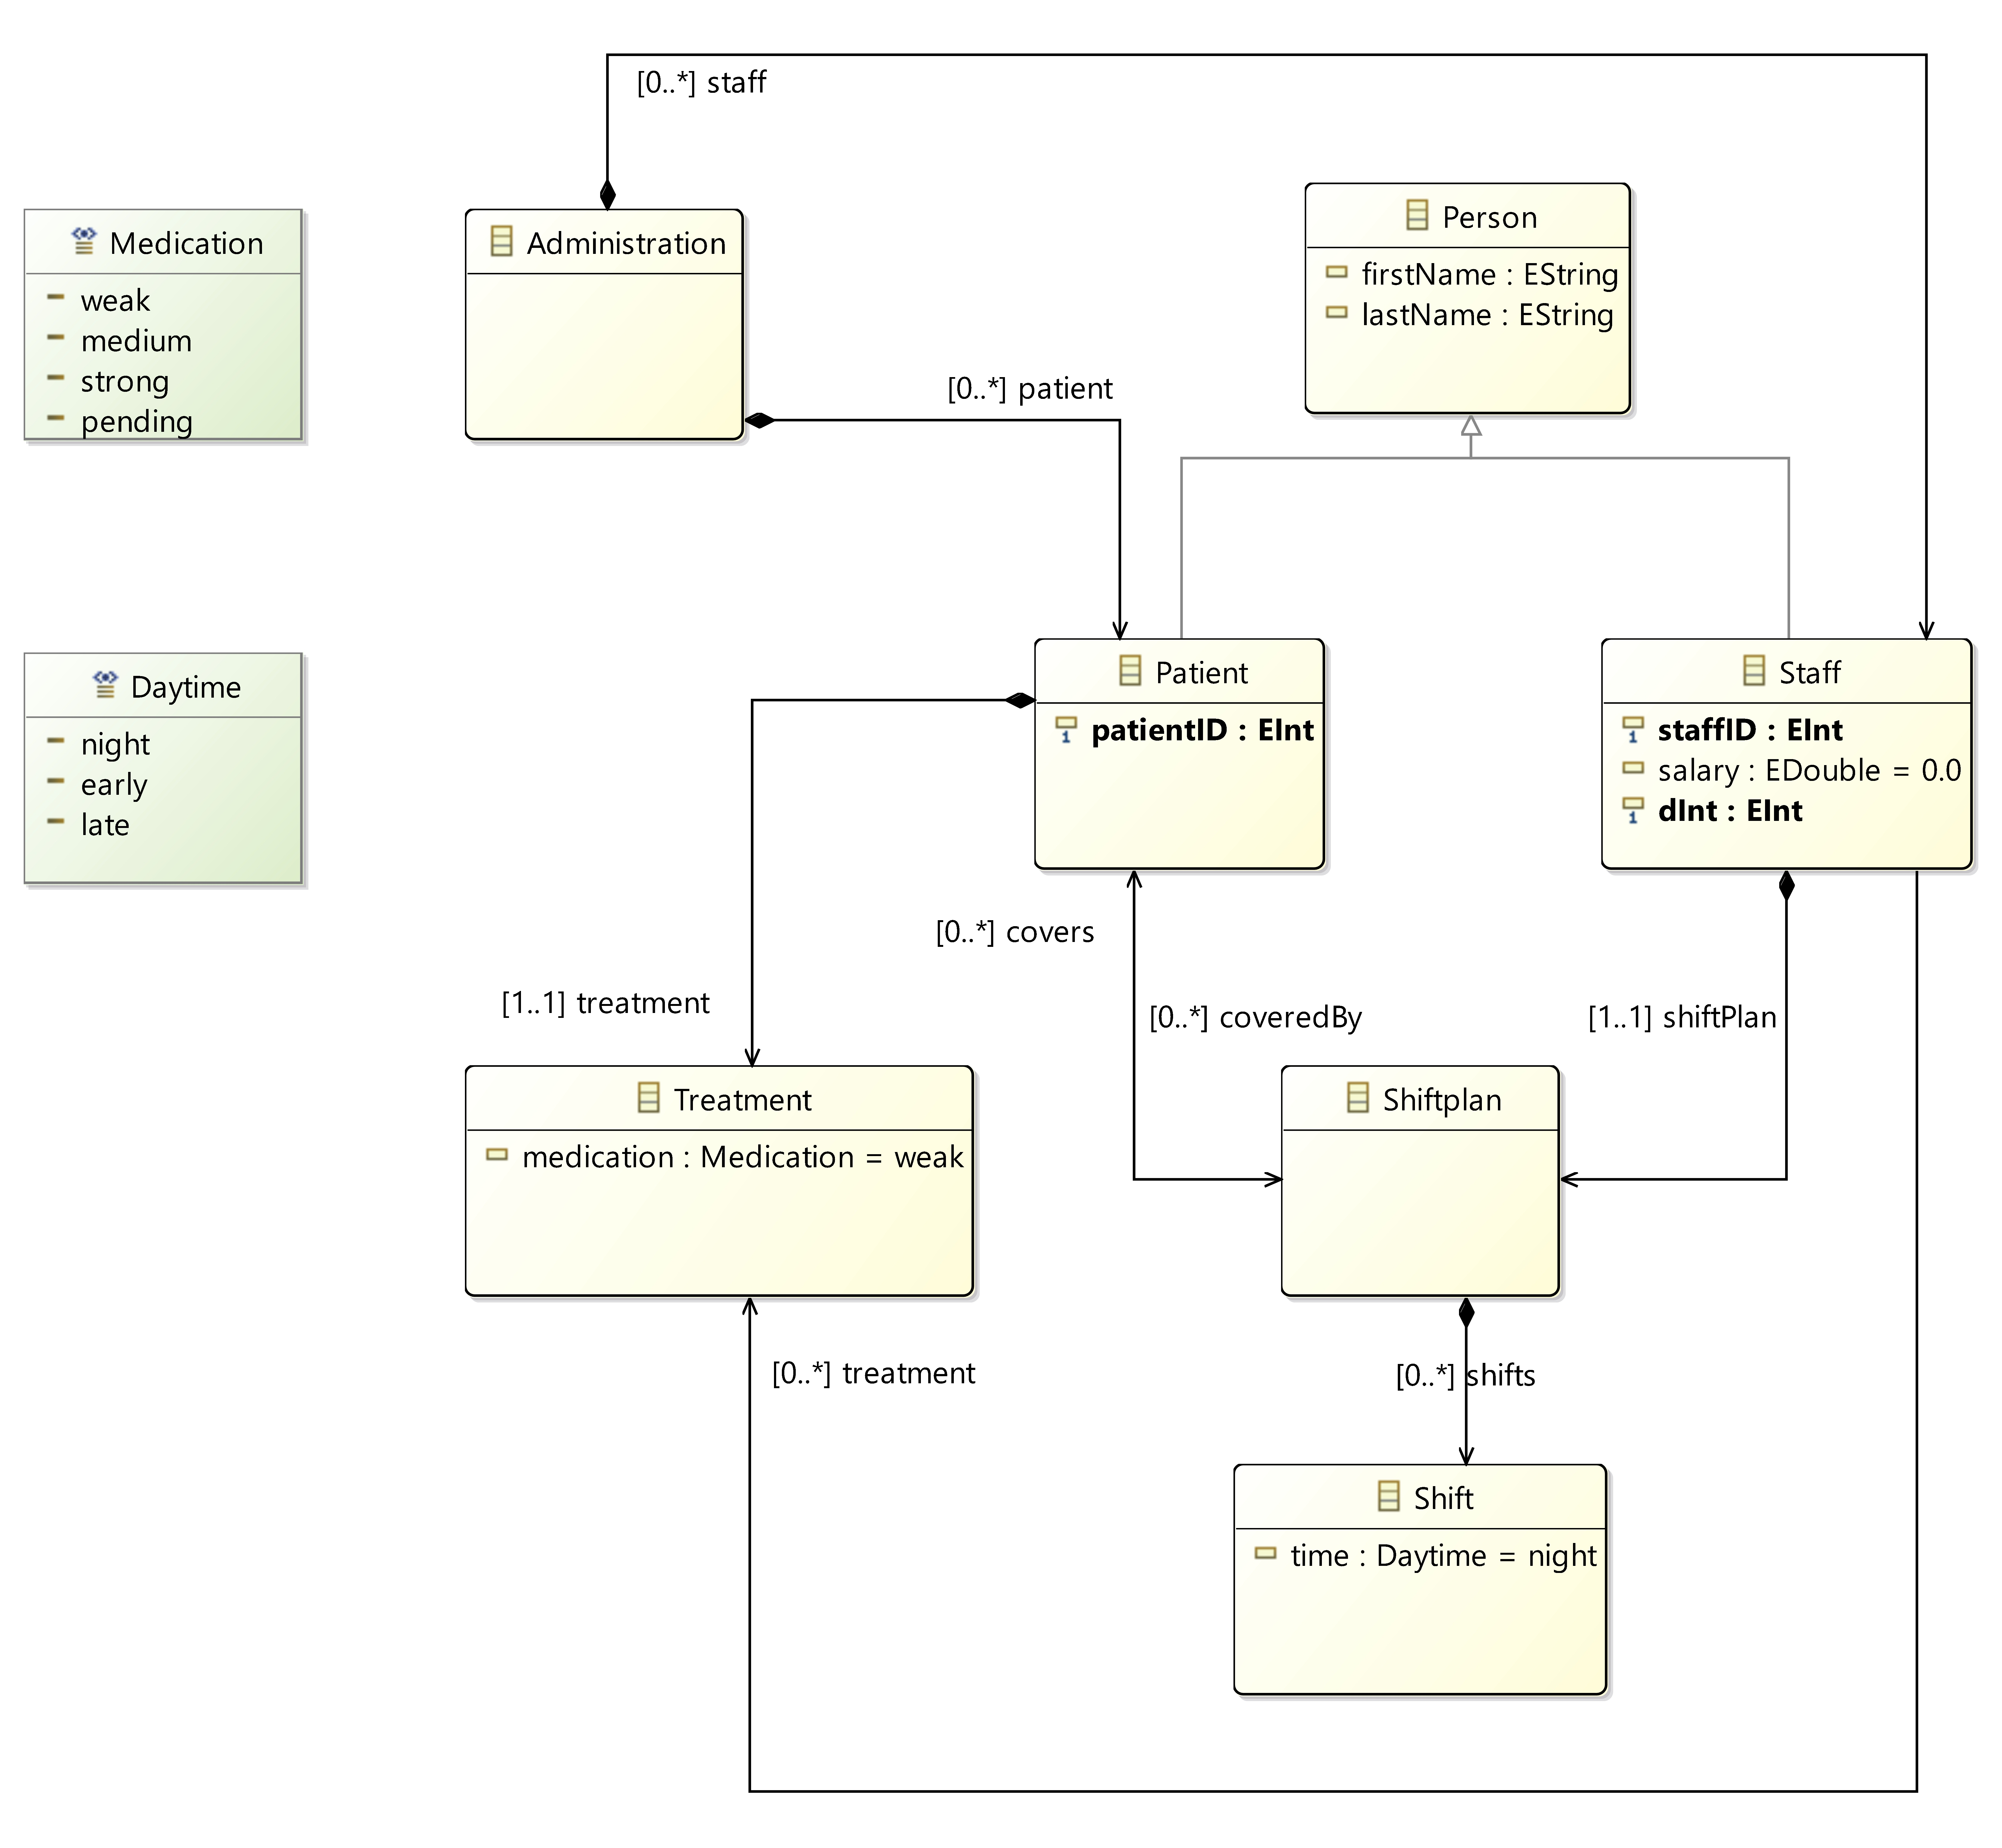
\includegraphics[scale=0.05 ]{pictures/AdministrationExample class diagram.jpg}
    \caption{\centering{Administration model}}
    \label{Administration model}
\end{figure}

\clearpage

For this purpose, we will be creating this new \textbf{administration metamodel} from scratch. If you do not want to exercise the creation of another metamodel yourself, you can skip this part and continue here with the \textbf{creation of a new TGG Project} in the next section.\newline

For our administration metamodel, we need the administration container first. So go ahead and create it \textbf{as we did it for the hospital}.\newline

\textbf{Persons:}

Then we need the persons which we want to cover for our administration. So, the next class you want to create are the \textbf{persons}, who should have a \textbf{first name} and a \textbf{last name} of the type \textbf{EString}.\newline

\textbf{Shifts:}

The two next classes are the \textbf{patients} and the \textbf{staff}, which are of the \textbf{ESuperType} person so both patients and staff members are extended by the persons and have names as well. For the staff, we also want additional information such as the \textbf{staffID}, a \textbf{salary}, and the \textbf{dInt} variable to indicate the department a staff member belongs to. A patient only needs a \textbf{patientID} as an additional attribute. After creating the two classes we need to connect them to the administration by adding a \textbf{staff relation} for the staff and \textbf{patient relation} for the patients.\newline

\textbf{Shiftplans:}

The next classes shiftplan and shift will be responsible for the coverage of the patients. So go ahead and create the class \textbf{Shiftplan} it does not require any attributes. But we want to add a \textbf{relation towards the staff} which ensures every staff member has \textbf{exactly one} shiftPan. Create the relation \textbf{shiftPlan} and set the upper and lower bounds to 1 to fulfill the desired multiplicities. We also want the patients to be covered by the shiftplan. Hence, we need a \textbf{bidirectional relation between the patients and the shift plans}.


The class \textbf{shift} will fill up a shiftPlan with shifts for the respective daytime. The times can be considered via the creation of the \textbf{Daytime Enumeration} with the literals \textbf{night}, \textbf{early}, and \textbf{late} and adding them as an attribute to the shifts class.\newline

\textbf{Medication and Treatment:}

After covering the care throughout the day, the treatment of patients is of importance as well. So, we need to create the \textbf{enumeration Medication} with the following four types: \textbf{weak}, \textbf{medium}, \textbf{strong}, and \textbf{pending}.

Then we have to create a class that includes the medication. Create the class \textbf{Treatment} and a \textbf{medication attribute} that accesses the medication enumeration. The last step we need to do is to \textbf{connect the treatment class to our staff and the patients}. \newline

The created metamodel should be completed now.

\subsection{Creating a TGG project}

%For this section, we will be using the \textbf{branch \textsf{EcoreOnly2}} from our Git repository.

%If you skipped the creation of the metamodel or you are unsure whether your model works correctly, please use this branch of our repository for the next section.\newline

We have now two metamodels containing information that are partly the same and partly different, but how do we connect the two sides and create a consistent triple? As a reminder, a consistent triple consists of three models which are related. The first model of a consistent triple is a so-called \textbf{source model}, which is represented by the hospital model in our case. The second model is the so-called \textbf{target model}, which is the administration model we have created in the previous segment. The third model is the \textbf{correspondence model} which puts the target and source model with each other.\newline

\textbf{Project creation:}

Let us start with creating a new TGG Project to link our hospital metamodel with the administration metamodel. To create a new TGG Project just click on button \ref{item:3} with the \textbf{green rhomb and the folder}. Then proceed with:\newline

\centering

Use the name \textsf{"Hospital2Administration"} → Select option \textsf{"Project with preselected metamodel"}

→ Press \textsf{"next"}

\clearpage

\raggedright

Now you have to select a \textbf{source metamodel} which will be the hospital example in our case. Scroll down through the list of possible options shown in the chart below  and select:\newline

\centering

\textcolor{Blue}{\textsf{platform:/resource/HospitalExample/model/HospitalExample.ecore}}\newline

\raggedright

\begin{figure}[h]
    \centering
    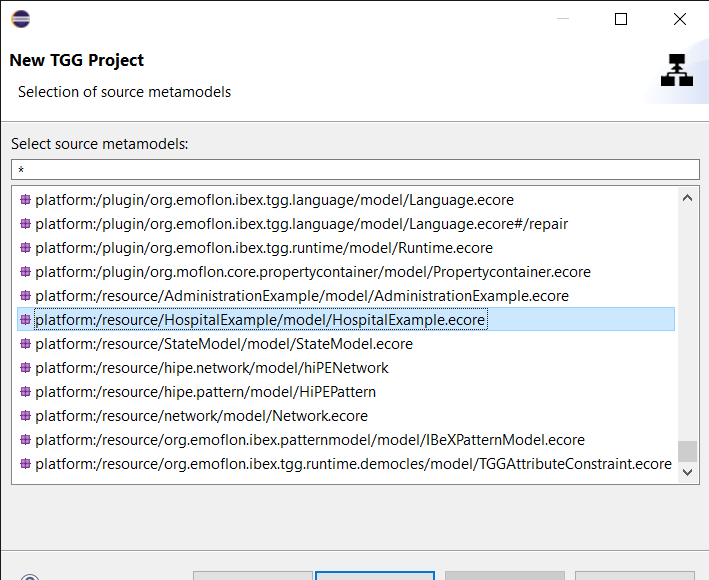
\includegraphics[scale=0.5 ]{pictures/selectSourceModel.png}
    \caption{\centering{Source model selection}}
    \label{Source model selection}
\end{figure}

The second model to select will be our \textbf{target model} and you might have already guessed it we will select our Administration metamodel: \newline

\centering

\textcolor{Blue}{\textsf{platform:/resource/AdministrationExample/model/AdministrationExample.ecore}}\newline

-> Afterwards press \textsf{"Finish"}\newline

\raggedright

Right now, we have a hospital metamodel and an administration metamodel but they are not connected. As a consequence, we need means to create relations between our two metamodels. These relations are defined in the files we will inspect now.

In the source folder you will find the \textbf{tgg package} and in it you will find the \textbf{Schema.tgg} file. This file is the central element linking both the source and the target side since it defines the \textbf{correspondence metamodel} for the connections between both the source and the target side. The correspondence metamodel defined by the Schema.tgg also completes our triple of metamodel graphs.\newline

\textbf{Warning:} Please always start the name of your project with a \textbf{capital letter}. The automatic file generation will not work otherwise.\newline

There are three important parts in the Schema file. Also there are a lot of desired elements missing in the Schema.tgg which will be added throughout the next section. Do not worry we will explain everything in detail and walk you through every step.
\clearpage

\subsection{Writing a TGG schema}

The automatically generated Schema.tgg should look like this:\newline

{\setstretch{1.2}

1\hspace{0.5cm}\textcolor{Purple}{\#\textit{import}} \textcolor{Orange}{"platform:/resource/AdministrationExample/model/AdministrationExample.ecore"}

2\hspace{0.5cm}\textcolor{Purple}{\#\textit{import}} \textcolor{Orange}{"platform:/resource/HospitalExample/model/HospitalExample.ecore"}

3\hspace{0.5cm}\textcolor{Purple}{\#\textit{schema}} Hospital2Administration

4\hspace{0.5cm}\colorbox{LightYellow}{\#\textit{source}} \{

5\hspace{1cm}HospitalExample

6\hspace{0.5cm}\}

7\hspace{0.5cm}\colorbox{LightSalmon}{\#\textit{target}}\{ 

8\hspace{1cm}AdministrationExample

9\hspace{0.5cm}\} 

10\hspace{0.5cm}\textcolor{Purple}{\#\textit{correspondence}} \{

11\hspace{0.5cm}\}

12\hspace{0.5cm}\textcolor{Purple}{\#\textit{attributeConditions}} \{
	
13\hspace{0.5cm}\} \newline

}

\textbf{Source and target model:}

First, the Schema.tgg defines the \textbf{source} and the \textbf{target} which was done automatically in our case because we defined the source and target model when we created the project. If you want to start with a blank project you have to do this yourself. You can see this definition in lines 4 to 9 where the \textsf{HospitalExample} metamodel was defined as the source model and the \textsf{AdministrationExample} metamodel was defined as the target model.\newline

\textbf{Correspondences:}

The second block consists of the \textbf{correspondences} between our meta models. The connections between our models we have talked previously about are called correspondences and their purpose is to define the elements which are connected. This might be a bit confusing so let us take a look at our example to make things clearer. The very first correspondence we want to create is the correspondence between our hospital and the administration. We can create a correspondence by writing the name of our correspondence and defining which elements on the source and target side should be connected in this correspondence. We recommend using the names of the elements we want to correspond with each other as the \textbf{names for the correspondence} for comprehensibility reasons.\newline

\textbf{Staff and patients:}

Go ahead and write \textsf{HospitalToAdministration} within the \textcolor{Purple}{\#\textit{correspondence}} bracket and \textbf{add curved brackets} to it.
Now we need to choose an element of the source/hospital side we want to correspond with an element on the target/administration side. As the name of the correspondence already indicates we want the \textbf{hospital class} to correspond with the \textbf{administration class} on the target metamodel.

A source element can be added via typing \textsf{\#src-> <nameOfElement>}. In the case of our hospital, we have to type \textsf{\#src->Hospital}.

Since we are still missing an element on the target side, we add the administration by writing \textsf{\#trg->Administration}. Our correspondence metamodel has now one correspondence between the hospital and the administration.\newline

However, we have still more elements we want to correspond with each other. Furthermore we want to connect the \textbf{staff} and the \textbf{patients} of both sides to each other. Let us create the new correspondence \textsf{StaffToStaff} and assign the staff classes of both sides as target and source to this correspondence.\newline

Try coding the \textsf{PatientToPatient} correspondence yourself. For the correspondence between patients, we want to connect the patients on the source side with their respective counterparts on the target side.

\clearpage

\textbf{Doctors and nurses:}

Now we have covered the rather obvious correspondences between our two models, but some classes contain information we want to be present in the other model too. We only have staff members on the target side but we still want to differentiate \textbf{doctors} from \textbf{nurses} there. Since we do know that the doctors and the nurses are related to the staff class on the source side, it makes sense to let the nurses and doctors correspond with the staff on the target side.

Let us create two further \textbf{correspondences} then. Firstly, we need the \textbf{DoctorToStaff} correspondences which ensures a doctor on the source side corresponds with the staff on the target side. Secondly, the nurses should correspond with staff in the same way, and hence we need the \textbf{NurseToStaff} correspondence.\newline

Finally your \textcolor{Purple}{\textit{\#correspondence}} section should look like this:\newline

{\setstretch{1.2}


10\hspace{0.5cm}\textcolor{Purple}{\#\textit{correspondence}} \{

11\hspace{1cm}HospitalToAdministration\{

12\hspace{1.5cm}\colorbox{LightYellow}{\#\textit{src->}}Hospital

13\hspace{1.5cm}\colorbox{LightSalmon}{\#\textit{trg->}}Administration

14\hspace{1cm}\}

15\hspace{1cm}StaffToStaff\{
	
16\hspace{1.5cm}\colorbox{LightYellow}{\#\textit{src->}}Staff

17\hspace{1.5cm}\colorbox{LightSalmon}{\#\textit{trg->}}Staff

18\hspace{1cm}\}

19\hspace{1cm}PatientToPatient\{

20\hspace{1.5cm}\colorbox{LightYellow}{\#\textit{src->}}Patient

21\hspace{1.5cm}\colorbox{LightSalmon}{\#\textit{trg->}}Patient

22\hspace{1cm}\}

23\hspace{1cm}DoctorToStaff\{

24\hspace{1.5cm}\colorbox{LightYellow}{\#\textit{src->}}Doctor

25\hspace{1.5cm}\colorbox{LightSalmon}{\#\textit{trg->}}Staff

26\hspace{1cm}\}

27\hspace{1cm}NurseToStaff\{

28\hspace{1.5cm}\colorbox{LightYellow}{\#\textit{src->}}Nurse

29\hspace{1.5cm}\colorbox{LightSalmon}{\#\textit{trg->}}Staff

30\hspace{1cm}\}

31\hspace{0.5cm}\}

}

\clearpage

\subsection{TGG Rules}

Since the ruleset and certain specifications for the triple grammar graph project are quite extensive, we do not want you to create everything by yourself but rather explain to you the ideas behind certain structures. For this reason there are two Hospital2Administration projects. \textbf{Hospital2AdministrationTemplate} is the template you should be using for this part of the tutorial. It contains all of the predefined stuff you need for it and you can just add the new stuff to it. \textbf{Hospital2AdministrationSolution} contains the solution for this part of the tutorial.\newline

\textbf{First rule:}

In contrast to the Schema.tgg where we defined the correspondence metamodel for the hospital and the administration, rules are responsible for the \textbf{creation of the actual structure} of our triple grammar graph. You will notice they work similarly to the rules we defined in the graph transformation project. Start with the creation of a new TGG rule in the package \textsf{org.emoflon.ibex.tgg.rules}.\newline

\textbf{Please create this rule in the described way.}\newline

\centering

Click on the package →  Press button \ref{tgg_rule} → Name it \textsf{"HospitalToAdministration"} → \textsf{"Finish"}\newline

\raggedright

\begin{figure}[h]
    \centering
    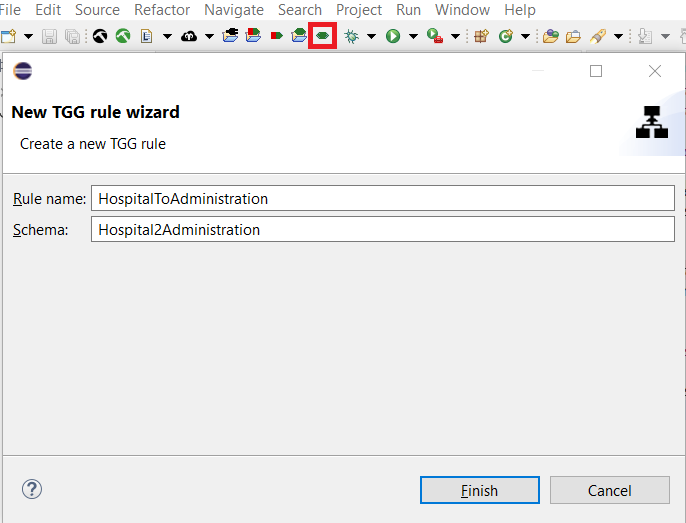
\includegraphics[scale=0.5 ]{pictures/tgg_rule_creation.png}
    \caption{\centering{TGG rule creation}}
    \label{TGG rule creation}
\end{figure}

As we can see the proper schema is assigned automatically, at least if you have selected the right package in your TGG project.\newline

For our first TGG rule, we want to create a connection for the hospital and the administration, as well as the nodes themselves. For this rule, we want a \textbf{hospital node} and a \textbf{reception node} with an \textbf{edge between them} on the source side.

The target side will require the creation of an \textbf{administration node}.

So far, the syntax of our TGG rule is almost the same as in graph transformation projects.\newline

According to the correspondence metamodel that we have defined in the Schema.tgg this rule also needs to consider the correspondence between our hospital node and the administration node. We do this by \textbf{adding a new correspondence} (lines 16 to 20) in the \textcolor{Purple}{\#correspondence} bracket.

This is similar to the principle of graph transformation rules. We first have define in the ecoremodel what relations different elements in our model have between each other, i.e references.
When creating instances of these elements via the application of a rule we also need to add an instance of those relations explicitly.

\clearpage

Please name the correspondence \textsf{htoa} and define its type as \textsf{HospitalToAdministration}. This is the correspondence we have created in the Schema.tgg. 

Now we are going to add the hospital node we have created in this rule to the source side and the administration node to the target side.\newline

Finally your rule should look like this: \newline

{\setstretch{1.2}

1\hspace{0.5cm}\colorbox{LightYellow}{\textit{\#source}}\{ 

2\hspace{1cm}\textcolor{LimeGreen}{++hospital:Hospital\{}

3\hspace{1.5cm}\textcolor{LimeGreen}{++-reception->reception}

4\hspace{1cm}\textcolor{LimeGreen}{\}}

5\hspace{1cm}\textcolor{LimeGreen}{++reception:Reception}

6\hspace{0.5cm}\}

7\hspace{0.5cm}\colorbox{LightSalmon}{\textit{\#target}}\{

8\hspace{1cm}\textcolor{LimeGreen}{++administration:Administration}

9\hspace{0.5cm}\}

10\hspace{0.5cm}\textcolor{Purple}{\textit{\#correspondence}}\{

11\hspace{1cm}\textcolor{LimeGreen}{++htoa:HospitalToAdministration\{}

12\hspace{1.5cm}\colorbox{LightYellow}{\textit{\#src->}}\textcolor{LimeGreen}{hospital}

13\hspace{1.5cm}\colorbox{LightSalmon}{\textit{\#trg->}}\textcolor{LimeGreen}{administration}

14\hspace{1cm}\textcolor{LimeGreen}{\}}

15\hspace{0.5cm}\}\newline

}

\begin{figure}[h]
    \centering
    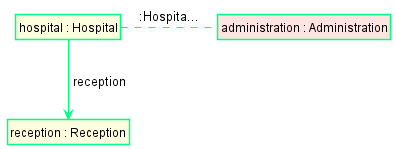
\includegraphics[scale=0.5 ]{pictures/h2a.png}
    \caption{\centering{PlantUML visualization HospitalToAdministration}}
    \label{TGG rule creation}
\end{figure}

\textbf{Note on the visualization}:

On the left side, we see our target side which creates the hospital and the reception and on the right side, we can see a new administration. The dotted line between the hospital and administration stands for the correspondence between the two models.\newline

Since you now have a grasp of how to create a rule let us take a step back and recapitulate its function. The rule creates a consistent triple consisting of the hospital and the reception nodes on the source side, the administration node on the target side, and their connection to each other in form of the correspondence. In other words, whenever we create a hospital and a reception on the source side, our correspondence requires the creation of an administration on the target side.

\clearpage

\textbf{Departments and rooms:}

The next two rules we will create are the rules for the departments and the rooms. 
The department rule creates a department with the respective edge to the hospital and works just as the departmentRule in the GT project. This rule allows the creation of a department if we already created a hospital node in our project. 

So go ahead and create a new tgg rule with the name \textsf{DepartmentRule} for which we need to add the following contents:\newline

{\setstretch{1.2}

1\hspace{0.5cm}\textcolor{Purple}{\textit{\#rule}} DepartmentRule \textcolor{Purple}{\textit{\#with}} Hospital2Administration

2\hspace{0.5cm}\colorbox{LightYellow}{\textit{\#source}} \{ 

3\hspace{1cm}h:Hospital \{

4\hspace{1.5cm}\hspace{1cm}\textcolor{LimeGreen}{++-department->department}

5\hspace{1cm}\}

6\hspace{1cm}\textcolor{LimeGreen}{++department:Department}

7\hspace{0.5cm}\}

8\hspace{0.5cm}\colorbox{LightSalmon}{\textit{\#target}} \{

9\hspace{0.5cm}\}

10\hspace{0.5cm}\textcolor{Purple}{\textit{\#correspondence}} \{

11\hspace{0.5cm}\}

12\hspace{0.5cm}\textcolor{Purple}{\textit{\#attributeConditions}} \{

13\hspace{1cm}incrementingDepartmentID(department.dID)

14\hspace{1cm}setDefaultNumber(department.maxRoomCount, \textcolor{Grey}{10})

15\hspace{0.5cm}\}\newline

}

\textbf{Note:}

We will explain the \textcolor{Purple}{\#attributeConditions} section later on. Please just copy these sections for now.\newline

\textbf{Please try to code the \textsf{RoomRule} yourself}.\newline

For this rule want to add a \textbf{room node} in case we have a department and assign the \textbf{default capacity} of that room to 4.

It should look like this in the end:\newline

{\setstretch{1.2}

1\hspace{0.5cm}\textcolor{Purple}{\textit{\#rule}} RoomRule \textcolor{Purple}{\textit{\#with}} Hospital2Administration

2\hspace{0.5cm}\colorbox{LightYellow}{\textit{\#source}} \{ 

3\hspace{1cm}department:Department\{

4\hspace{2cm}\textcolor{LimeGreen}{++-rooms->room}

5\hspace{1cm}\}

6\hspace{1cm}\textcolor{LimeGreen}{++room:Room\{}

7\hspace{2cm}capacity := \textcolor{Grey}{4}

8\hspace{1cm}\textcolor{LimeGreen}{\}}

9\hspace{0.5cm}\}

10\hspace{0.5cm}\colorbox{LightSalmon}{\textit{\#target}} \{

11\hspace{0.5cm}\}

12\hspace{0.5cm}\textcolor{Purple}{\textit{\#correspondence}} \{

13\hspace{0.5cm}\}

14\hspace{0.5cm}\textcolor{Purple}{\textit{\#attributeConditions}} \{

15\hspace{0.5cm}\} \newline

}

As you can see, we are only operating on the source side of our consistent triple since we do not have and do not need a correspondence for these elements on the target side because these elements are not present on the administration side. \newline

\clearpage

\textbf{Abstract rules:}

Let us continue with the remaining rules since we are still lacking the personnel and the patients. Look at the \textsf{StaffToStaffRule} which is already present in your Java project. Its visualization is shown in the chart below.

For this rule, we assume that a hospital node, at least one department node, an administration node and the correspondence between source and target side exist.

Then we want to create a staff node and its respective connections on the source side. When creating a staff node on the target side we also want to connect them to the target side by creating the \textsf{StaffToStaff} \textbf{correspondence} and the staff for the target side itself.

Upon creating a staff member on the target side, we also want to assign them a shift plan and a shift.

\begin{figure}[h]
    \centering
    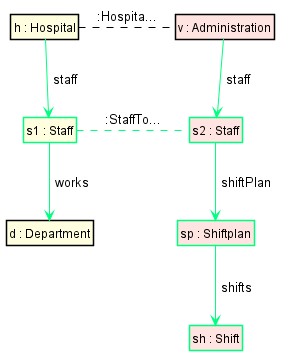
\includegraphics[scale=0.6 ]{pictures/StaffToStaffRule.png}
    \caption{\centering{PlantUML visualization StaffToStaffRule}}
    \label{TGG rule creation}
\end{figure}

You probably have noticed the keyword \textcolor{Purple}{\#abstract} in the definition of this rule. Similar to \textbf{abstract} rules from graph transformations this means that this rule cannot be applied directly.\newline

\textbf{Extending abstract rules:}

You might also wonder how we are going to distinguish doctors from nurses in the administration view. That is the part where the \textsf{DoctorToStaff} and \textsf{NurseToStaff} \textbf{correspondences} that we have created previously come into play. With those we have established a correspondence between doctors and nurses on the source side to staff on the target side.

This requires a further extension of our Staff rule which can be added just below the \textsf{StaffToStaffRule}. The keyword for the further specification of an existing rule in TGG is \textcolor{Purple}{\#extends} which needs to be added after the name of the rule. If you remember from the GT part of our tutorial the keyword \textcolor{Purple}{\#extends} works similar to the concept of inheritance in Java. We reduce redundancies for the new rules because they inherit the elements defined in the \textsf{StaffToStaffRule} as well.
For the creation of the DocToStaff rule, which can be done in the present StaffToStaff rule, we need to add a staff node of the type doctor on our \colorbox{LightYellow}{\textit{\#source}} side and a new staff node on the \colorbox{LightSalmon}{\textit{\#target}} side. \newline

{\setstretch{1.2}

1\hspace{0.5cm}\textcolor{Purple}{\textit{\#rule}} DocToStaffRule \textcolor{Purple}{\textit{\#extends}} StaffToStaffRule \textcolor{Purple}{\textit{\#with}} Hospital2Administration

2\hspace{0.5cm}\colorbox{LightYellow}{\textit{\#source}}\{

3\hspace{1cm}\textcolor{LimeGreen}{++s1:Doctor}

4\hspace{0.5cm}\}

5\hspace{0.5cm}\colorbox{LightSalmon}{\textit{\#target}}\{

6\hspace{1cm}\textcolor{LimeGreen}{++s2:Staff}

7\hspace{0.5cm}\}

8\hspace{0.5cm}\textcolor{Purple}{\textit{\#correspondence}}\{

9\hspace{0.5cm}\}

10\hspace{0.42cm}\textcolor{Purple}{\textit{\#attributeConditions}}\{

11\hspace{1cm}doctorsalary(s2.salary)

12\hspace{0.5cm}\}\newline

}

\clearpage

The \textsf{NurseToStaffRule} can be created similarly. Please try it yourself before having a look at the syntax below. Change the type of staff member accordingly and adjust the attribute condition to \textsf{nursesalary}.\newline

{\setstretch{1.2}

1\hspace{0.5cm}\textcolor{Purple}{\textit{\#rule}} NurseToStaffRule \textcolor{Purple}{\textit{\#extends}} StaffToStaffRule \textcolor{Purple}{\textit{\#with}} Hospital2Administration

2\hspace{0.5cm}\colorbox{LightYellow}{\textit{\#source}}\{

3\hspace{1cm}\textcolor{LimeGreen}{++s1:Nurse}

4\hspace{0.5cm}\}

5\hspace{0.5cm}\colorbox{LightSalmon}{\textit{\#target}}\{

6\hspace{1cm}\textcolor{LimeGreen}{++s2:Staff}

7\hspace{0.5cm}\}

8\hspace{0.5cm}\textcolor{Purple}{\textit{\#correspondence}}\{

9\hspace{0.5cm}\}

10\hspace{0.42cm}\textcolor{Purple}{\textit{\#attributeConditions}}\{

11\hspace{1cm}nursesalary(s2.salary)

12\hspace{0.5cm}\}\newline

}

\begin{figure}[h]
    \centering
    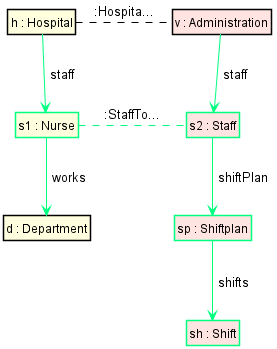
\includegraphics[scale=0.65 ]{pictures/NurseToStaffRule.png}
    \caption{\centering{Visualization of NurseToStaffRule. DocToStaffRule is similar with changed staff type.}}
    \label{NurseToStaffRule}
\end{figure}

\textbf{Shiftplan rule:}

The next function we want to cover is the shift plans. In the \textsf{ShiftplanRule}, we want to add an edge on the target side to make sure a patient is covered by a shift plan. So let us start by creating the new rule \textsf{ShiftPlanRule}.\newline

First, we want to make that rule \textbf{abstract} because as we have defined it in the GT part of our tutorial the coverage of patients via doctors and nurses works differently. While doctors are assigned to a patient directly, nurses cover patients indirectly with the rooms they are responsible for.

We require patient and staff nodes on the source side while having a staff, shift, shift plan and a patient node on the target side. Furthermore this shift plan has to be related to the specific staff and shift nodes via an edge.

For the patient node in our administration model, we want to add an edge to the shift plan to indicate a patient is covered in that shift plan.

In the last step for this rule, we need to define the \textbf{correspondences} with patients and staff members between the source and the target side. Since we have all elements on both sides defined this step should be pretty forward.\newline

You can look at the complete rule on the next page.

\clearpage

{\setstretch{1.2}

1\hspace{0.5cm}\textcolor{Purple}{\textit{\#abstract}} \textcolor{Purple}{\textit{\#rule}} ShiftplanRule \textcolor{Purple}{\textit{\#with}} Hospital2Administration

2\hspace{0.5cm}\colorbox{LightYellow}{\textit{\#source}} \{

3\hspace{1cm}p1:Patient\{\}

4\hspace{1cm}s1:Staff\{\}
	
5\hspace{0.5cm}\}

6\hspace{0.5cm}\colorbox{LightSalmon}{\textit{\#target}} \{
	
7\hspace{1cm}s2:Staff\{

8\hspace{1.5cm}-shiftPlan->sp

9\hspace{1cm}\}

10\hspace{1cm}sp:Shiftplan\{

11\hspace{1.5cm}-shifts->sh

12\hspace{1cm}\}

13\hspace{1cm}sh:Shift

14\hspace{1cm}p2:Patient\{

15\hspace{1.5cm}\textcolor{LimeGreen}{++-coveredBy->sp}

16\hspace{1cm}\}

17\hspace{0.5cm}\}

18\hspace{0.5cm}\textcolor{Purple}{\textit{\#correspondence}} \{
		
19\hspace{1cm}pToP:PatientToPatient\{

20\hspace{1.5cm}\colorbox{LightYellow}{\textit{\#src->}}p1

21\hspace{1.5cm}\colorbox{LightSalmon}{\textit{\#trg->}}p2

22\hspace{1cm}\}

23\hspace{1cm}sToS:StaffToStaff\{

24\hspace{1.5cm}\colorbox{LightYellow}{\textit{\#src->}}s1

25\hspace{1.5cm}\colorbox{LightSalmon}{\textit{\#trg->}}s2

26\hspace{1cm}\}
	
27\hspace{0.5cm}\}

28\hspace{0.5cm}\textcolor{Purple}{\textit{\#attributeConditions}} \{

29\hspace{0.5cm}\} \newline

}

\textbf{Specific shiftplans:}

For this case, we also need differentiation between doctors and nurses, due to the different paths towards the coverage of a patient. Hence, we need two more rules.

These are already given in your project. You can look at the respective visualization of the \textsf{DoctorShiftplanRule} and the \textsf{NurseShiftplanRule} in your project: \newline

\begin{figure}[h]
    \centering
    
    \begin{subfigure}[b]{0.3\textwidth}
    
    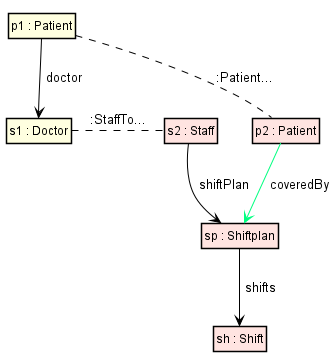
\includegraphics[scale=0.45 ]{pictures/DocShiftplanRule.png}
    \caption{\centering{Visualization of DocShiftplanRule}}
    \label{DocShiftplanRule}
    
    \end{subfigure}\hspace{2cm}
    \begin{subfigure}[b]{0.3\textwidth}
    
    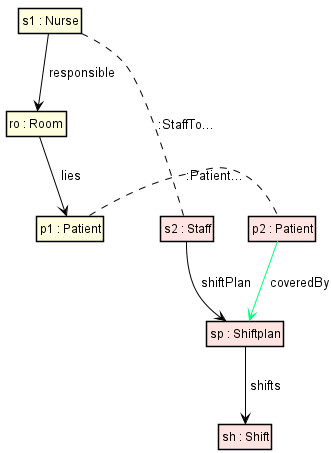
\includegraphics[scale=0.45 ]{pictures/nurseShiftPlan.png}
    \caption{\centering{Visualization of NurseShiftplanRule}}
    \label{NurseShiftplanRule}
    
    \end{subfigure}
    
\end{figure}

\clearpage

\textbf{Rules regarding patients:}

Now that we have covered the staff and their respective shifts, we need to handle the patients. 

The \textbf{abstract} \textsf{PatientToPatientRule} adds patients and the required correspondences for further rules.

This rule is already given in the project and you might want to take a look at it. The visualization is shown in the chart below:

\begin{figure}[h]
    \centering
    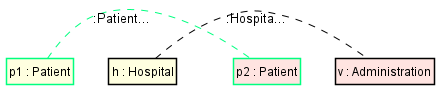
\includegraphics[scale=0.65 ]{pictures/patientToPatient.png}
    \caption{\centering{Visualization of PatientToPatientRule}}
    \label{PatientToPatientRule}
\end{figure}

As you might have noticed we are adding two correspondences to our model which are independent from each other. This requires us to add two rules extending the \textsf{\textit{PatientToPatient}} rule to fit the patients into our hospital view.

For the first rule, we assume that our patients are waiting in the reception until they are moved to a room where they are treated. So, we want to create the rule \textsf{PatientInReception} where we require the context of the hospital node, the edge towards the reception and the reception node on the source side. Additionally, we require the context of the administration node and the \textsf{HospitalToAdministration} correspondence between the hospital node and the administration node. 

Regarding the creation of nodes and edges, we want to add a patient node and a \textsf{waits} edge from the reception to the patient on the source side.

For the target side, we want to create the patient node and its respective edge from the administration towards the patient node.\newline

\textbf{Please try creating this rule yourself, the syntax can be found below:}\newline

{\setstretch{1.2}

1\hspace{0.5cm}\textcolor{Purple}{\textit{\#rule}} PatientInReception \textcolor{Purple}{\textit{\#extends}} PatientToPatient \textcolor{Purple}{\textit{\#with}} Hospital2Administration

2\hspace{0.5cm}\colorbox{LightYellow}{\textit{\#source}} \{ 

3\hspace{1cm}\textcolor{LimeGreen}{++ p1 : Patient}

4\hspace{1cm}h:Hospital\{

5\hspace{1.5cm}-reception->r

6\hspace{1cm}\}

7\hspace{1cm}r:Reception\{

8\hspace{1.5cm}\textcolor{LimeGreen}{++-waits->p1}

9\hspace{1cm}\}

10\hspace{0.5cm}\}

11\hspace{0.5cm}\colorbox{LightSalmon}{\textit{\#target}} \{

12\hspace{1cm}\textcolor{LimeGreen}{++ p2 : Patient}

13\hspace{1cm}v:Administration\{

14\hspace{1.5cm}\textcolor{LimeGreen}{++-patient->p2}

15\hspace{1cm}\}

16\hspace{0.5cm}\}

17\hspace{0.5cm}\textcolor{Purple}{\textit{\#correspondence}} \{
	
18\hspace{1cm}htov:HospitalToAdministration\{

19\hspace{1.5cm}\colorbox{LightYellow}{\textit{\#src->}}h
			
20\hspace{1.5cm}\colorbox{LightSalmon}{\textit{\#trg->}}v

21\hspace{1cm}\}

22\hspace{0.5cm}\}

23\hspace{0.5cm}\textcolor{Purple}{\textit{\#attributeConditions}} \{

24\hspace{0.5cm}\}

}

\clearpage

The second rule \textsf{PatientInRoom} is already given in your project. This rule adds the \textsf{lies} edge from the context node \textsf{room} to the node \textsf{patient}.\newline

Its visualization is depicted in the chart below:

\begin{figure}[h]
    \centering
    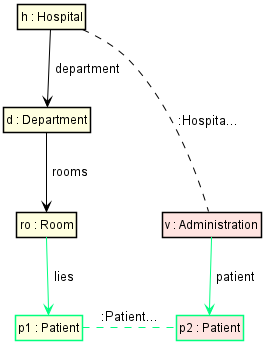
\includegraphics[scale=0.65 ]{pictures/PatientInRoomRule.png}
    \caption{\centering{Visualization of PatientInRoomRule}}
    \label{PatientInRoomRule}
\end{figure}

\textbf{NurseToRoomRule:}

The last remaining rule is the \textsf{NurseToRoomRule}, where we add the edge from the nurse node to the room node according to the assumptions in our metamodel. The rule is also given in your project and the visualization is depicted in the chart below:

\begin{figure}[h]
    \centering
    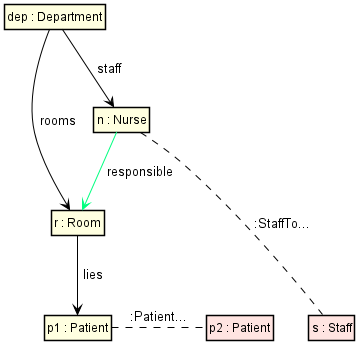
\includegraphics[scale=0.65 ]{pictures/NurseToRoomRule.png}
    \caption{\centering{Visualization of PatientInRoomRule}}
    \label{PatientInRoomRule}
\end{figure}

After creating the rules for the infrastructure and the persons in the hospital you should have a grasp of the concept of creating rules for triple graph grammars and the way they are working. So let us continue with another important function we have skipped previously, the \textbf{attribute conditions}. 

\clearpage

\subsection{Attribute Conditions}

In this chapter we will be covering \textbf{attribute conditions}. Attribute conditions can be used to assign meaningful values to attributes when creating a coherent graph triplet. They can also modify already set attribute values of an existing target and source graph pair to synchronize them.

They will be applied when their corresponding rule is.\newline

You have already seen how to invoke them in the previous chapters:

{\setstretch{1.2}

\hspace{0.5cm}...

\hspace{0.5cm}\textcolor{Purple}{\textit{\#attributeConditions}} \{

\hspace{1cm}incrementingDepartmentID(department.dID)

\hspace{1cm}setDefaultNumber(department.maxRoomCount, \textcolor{Grey}{10})

\hspace{0.5cm}\} \newline

}

To introduce you to the inner workings of attribute conditions we will have a look a the pre-defined condition \textsf{setDefaultNumber(variableNumber:EDouble, defaultNumber:EDouble)}.\newline

Please, go to \textbf{line 75} in this file:

\begin{figure}[h]
    \centering
    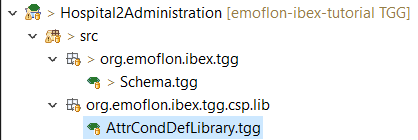
\includegraphics[scale=0.65 ]{pictures/locSetDefaultNumber.png}
    \caption{\centering{Location of \textsf{setDefaultNumber}}}
    \label{setDefaultNumber}
\end{figure}

This file contains the library of predefined attribute conditions. Let us inspect the setDefaultNumber condition which was used previously. This attribute condition ensures that an attribute value is set to a defined default number if it is unset. \newline

\textbf{Control flow:}

Attribute conditions in general
use a control flow that will be defined and is implemented as a \textbf{switch case}. Each case condition is made up by \textbf{all valid combinations of the bounding states} of referenced attribute values, i.e the input parameters.\newline

An attribute can be \textbf{free} meaning that there is no value assigned to it. This will be represented as "\textcolor{Purple}{F}" in the condition.

The other option is that the attribute is \textbf{bonded} which means that it already has a set value. This will be represented as "\textcolor{Purple}{B}" in the condition.

These cases will be defined in the definition of the attribute condition.\newline

Note that there are two different sets of cases for the two application scenarios:

\begin{itemize}
    \item\textcolor{Purple}{\textit{\#sync}}: Keeping two existing graphs synchronized. [\textcolor{Purple}{ F F } ... \textcolor{Purple}{ F}] is not available since unset values don't need to be synchronized.
    \item\textcolor{Purple}{\textit{\#gen}}: Generation of a new graph pair.
\end{itemize}

\clearpage

\textbf{Pre-defined conditions:}

Let's have a look at the definition of \textsf{setDefaultNumber}:\newline

{\setstretch{1.2}

75\hspace{0.5cm}setDefaultNumber(variableNumber:EDouble, defaultNumber:EDouble) \{

76\hspace{1cm}\textcolor{Purple}{\textit{\#sync}}: [\textcolor{Purple}{\textit{B B}}], [\textcolor{Purple}{\textit{F B}}]

77\hspace{1cm}\textcolor{Purple}{\textit{\#gen}}: [\textcolor{Purple}{\textit{B B}}], [\textcolor{Purple}{\textit{F B}}], [\textcolor{Purple}{\textit{F F}}]

78\hspace{0.5cm}\}\newline

}

Because this condition is pre-defined the effects of each case are already implemented. If an attribute has no value and is perceived as free, it would be assigned the \textsf{defaultNumber:EDouble} we defined in the attribute condition of our rule. If the \textsf{variableNumber:EDouble} is already set and hence bound, the bound variableNumber will be kept.

Note that there is no case [\textcolor{Purple}{B F}] because a default value has to be specified for this to work.\newline

You can find a comprehensive list of the predefined attribute conditions and a short explanation of each condition in the \textbf{appendix}.\newline

\textbf{User-defined conditions:}

To create a user-defined attribute condition you have to define it in the \textsf{schema.tgg} first. Let us start with by inspecting the \textsf{incrementingDepartmentID} which is already given:\newline

{\setstretch{1.2}

88\hspace{0.5cm}\textcolor{Purple}{\textit{\#userDefined}} incrementingDepartmentID(id:EInt) \{
	
89\hspace{1cm}\textcolor{Purple}{\textit{\#sync}}:\hspace{0.3cm}[\textcolor{Purple}{\textit{B}}], [\textcolor{Purple}{\textit{F}}]
		
90\hspace{1cm}\textcolor{Purple}{\textit{\#gen}}:\hspace{0.3cm}[\textcolor{Purple}{\textit{F}}]
		
91\hspace{0.5cm}\}\newline
}

A user-defined attribute condition is defined by the keyword \textcolor{Purple}{\#userDefined} followed by the \textbf{name} of the attribute condition and the \textbf{parameters/attributes} to alter.

In our case, we want to modify the ID of a department. The different boundary states are defined in the curved brackets just like in the predefined attribute conditions.

Now head to the \textsf{.constraints.custom.hospital2administration} package and open up the \textsf{UserDefined\_incrementingDepartmentID}. Which should look like this: \newline

{\setstretch{1.2}

1\hspace{0.5cm}\textcolor{Purple}{public class}
UserDefined\_incrementingDepartmentID \textcolor{Purple}{extends} RuntimeTGGAttributeConstraint

2\hspace{0.5cm}\{\hspace{0.5cm}	\textcolor{Purple}{private static int} \textcolor{Blue}{\textit{idIncrement}} = 1;

3\hspace{1cm}\textcolor{Grey}{@Override}

4\hspace{1cm}\textcolor{Purple}{public void} solve() \{

5\hspace{1.5cm}\textcolor{Purple}{if} (\textcolor{Blue}{variables}.size() != 1)

6\hspace{2cm}\textcolor{Purple}{throw new} RuntimeException("\textcolor{Blue}{The CSP -INCREMENTINGDEPARTMENTID- needs exactly 1 variables}");

7

8\hspace{1.5cm}RuntimeTGGAttributeConstraintVariable \textcolor{Tan}{v0} = \textcolor{Blue}{variables}.get(0);

9\hspace{1.5cm}String \textcolor{Tan}{bindingStates} = getBindingStates(\textcolor{Tan}{v0});

10

11\hspace{1.5cm}\textcolor{Purple}{switch}(\textcolor{Tan}{bindingStates}) \{

12\hspace{1.5cm}\textcolor{Purple}{case} "\textcolor{Blue}{F}":

13\hspace{2cm}\textcolor{Tan}{v0}.bindToValue(\textcolor{Blue}{\textit{idIncrement}}++);

14\hspace{2cm}setSatisfied(\textcolor{Purple}{true});

15\hspace{2cm}\textcolor{Purple}{break};

16\hspace{1.5cm}\textcolor{Purple}{case} "\textcolor{Blue}{B}":

17\hspace{2cm}setSatisfied(\textcolor{Purple}{true});

18\hspace{2cm}\textcolor{Purple}{return};

19\hspace{1.5cm}\textcolor{Purple}{default}: \textcolor{Purple}{throw new} UnsupportedOperationException("\textcolor{Blue}{This case in the constraint has not been implemented yet: }" + \textcolor{Tan}{bindingStates});

}

\clearpage

In line 2 we define the initial value of our department ID in the static variable \textsf{idIncrement}. Which will be incremented later on in the switch statement in lines 13 to 14.

If the department ID is free which is given as the parameter \textsf{id} in our attribute condition we switch to the \textcolor{Purple}{case} \textsf{"\textcolor{Purple}{F}"} and bind the ID to the value of the \textsf{idIncrement} variable. Afterwards we increasing this variable to give each department an unique ID.

In the next line, we set the boolean variable \textsf{setSatisfied} to \textsf{true} to fulfill the requirement for our runtime variable.

For the second \textcolor{Purple}{case} \textsf{“\textcolor{Purple}{B}”} we just set the setSatisfied value to true, since a department already has an ID and does not need one. \newline

Be aware that after the application of an attribute condition all involved attributes have to be \textbf{bound}.\newline

Maybe we should practice a bit by creating a fresh user-defined attribute condition. Our rooms also have IDs that we want to assign identically to the departmentIDs. Start by defining the attribute constraint \textsf{incrementingRoomID} in the \textsf{schema.tgg}. Its definition should look very similar:\newline

{\setstretch{1.2}

108\hspace{0.5cm}\textcolor{Purple}{\textit{\#userDefined}} incrementingRoomID(id:EInt)

109\hspace{0.5cm}\{
	
110\hspace{1cm}\textcolor{Purple}{\textit{\#sync}}:[\textcolor{Purple}{B}],[\textcolor{Purple}{F}]
		
111\hspace{1cm}\textcolor{Purple}{\textit{\#gen}}:[\textcolor{Purple}{F}]
		
112\hspace{0.5cm}\}\newline

}

Please \textbf{build} the project by pressing either the \textbf{black or the green hammer button} \ref{item:0} in the eMoflon Toolbar. Once you refresh your project folder you can see that the new attribute condition was created automatically and tucked into our project by eMoflon.

Now we have to implement the user-defined attribute constraint to do what it is supposed to do.
For this condition we want the same implementation logic as for \textsf{incrementingDepartmentID}.\newline

\textbf{Please try to implement the corresponding file in the \textsf{org.emoflon.ibex.tgg.operational.csp.constraints.custom.hospital2administration} package.} \newline

\textbf{Complex conditions:}

To further get to know user-defined attribute constraints let us look at the \textsf{UserDefined\_nametoname.Java} file which is a rather complex condition and already given in our project. As you can see in the schema.tgg the number of different boundary states has increased notably since we are handling more parameters. \newline

{\setstretch{1.2}

82\hspace{0.45cm}\textcolor{Purple}{\textit{\#userDefined}} nametoname(separator:EString, leftWord:EString, rightWord:EString, result:EString) \{

83\hspace{1cm}\textcolor{Purple}{\textit{\#sync}}: [\textcolor{Purple}{\textit{B B B B}}], [\textcolor{Purple}{\textit{B B B F}}], [\textcolor{Purple}{\textit{B B F B}}], [\textcolor{Purple}{\textit{B F F B}}], [\textcolor{Purple}{\textit{B F B B}}]
		
84\hspace{1cm}\textcolor{Purple}{\textit{\#gen}}: [\textcolor{Purple}{\textit{B B B B}}] , [\textcolor{Purple}{\textit{B B B F}}], [\textcolor{Purple}{\textit{B B F B}}], [\textcolor{Purple}{\textit{B F F B}}], [\textcolor{Purple}{\textit{B F B B}}], [\textcolor{Purple}{\textit{B F B F}}], [\textcolor{Purple}{\textit{B B F F}}], [\textcolor{Purple}{\textit{B F F F}}]

85\hspace{0.45cm}\} \newline
	
}

We should start by explaining the purpose of this attribute constraint. If you compare the name attributes of the patients and staff members in the hospital metamodel with the name attribute of the Person class in the administration metamodel, you will notice that the name attributes on the administration side are split up in first and last name. This specification forces us to split up the full name consisting of first and last name on the hospital side into two attributes if we want to propagate the name information from the hospital side to the administration side or concatenate two names if we want to execute the opposite operation. This leads to the four parameters we need for the attribute constraint.

The \textsf{separator:EString} defines the character we are using to distinguish first from last name in case both are in the same attribute. The \textsf{leftWord:EString} will define the first name while \textsf{rightWord:EString} will be handling the last name. The \textsf{result:EString} combines the three previous Strings to one String. \newline

\clearpage

If you open the java file of the attribute constraint you can see two arrays with sample names which we are using to generate a random first and last name whenever we invoke the attribute constraint, and the name attributes are not set yet:\newline

{\setstretch{1.2}

25\hspace{0.5cm}\textcolor{Purple}{case} \textcolor{Blue}{"BFFF"}:

26		  		

27\hspace{1cm}String \textcolor{Tan}{firstName} = firstNames[\textcolor{Tan}{random}.nextInt(\textcolor{Tan}{firstNames}\textcolor{Blue}{.length})];

28\hspace{1cm}\textcolor{Tan}{v1}.bindToValue(\textcolor{Tan}{firstName});

29\hspace{1cm}String \textcolor{Tan}{lastName} = \textcolor{Tan}{lastNames}[\textcolor{Tan}{random}.nextInt(\textcolor{Tan}{lastNames}\textcolor{Blue}{.length})];

30\hspace{1cm}\textcolor{Tan}{v2}.bindToValue(\textcolor{Tan}{lastName});

31\hspace{1cm}\textcolor{Tan}{v3}.bindToValue(\textcolor{Tan}{firstName} + \textcolor{Tan}{v0}.getValue() + \textcolor{Tan}{lastName});

32\hspace{1cm}setSatisfied(\textcolor{Purple}{true});	

33\hspace{1cm}\textcolor{Purple}{break}; \newline

}

For the case above we want a bound separator character which is a blank space in our case. Then we select a random first name from our first name array and bind its value to the runtime variable \textsf{v1} which represents the \textbf{leftWord}.

The same is done for the last name.

\textsf{v3} is the result of combining the values of the previous runtime variables.\newline

As you can see the user-defined constraints are a powerful way to create constraints that are not covered by our predetermined library.

\subsection{Running the TGG Project}

Now that we have finally defined all the elements and their respective correspondences of our models it is time to get back to our primary goal for this part of the tutorial. The generation of a consistent triple and its consistency maintenance.\newline

As a short reminder: A consistent triple includes the source model, a correspondence model, and a target model. Once information changes in one model we want to propagate the information to the other models to achieve consistency. eMoflon provides a different set of Java applications for this purpose and we will go through the important ones step by step. \newline

Open the package \textsf{org.emoflon.ibex.tgg.run.hospital2administration} and take a look at the different java applications you can see in the chart below:

\begin{figure}[h]
    \centering
    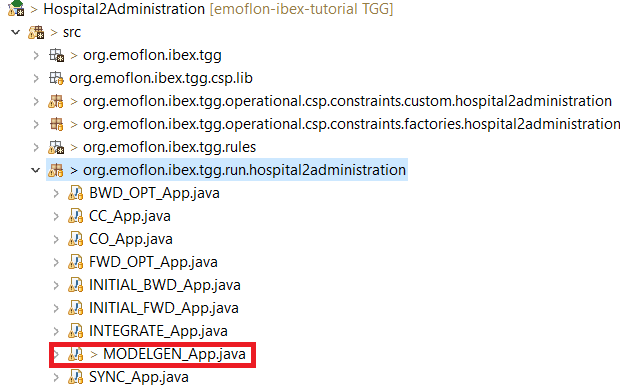
\includegraphics[scale=0.65 ]{pictures/modelGENApp.png}
    \caption{\centering{run.hospital2administration package}}
    \label{setDefaultNumber}
\end{figure}

\clearpage

The first operation we are interested in is the \textit{\textsf{MODELGEN\_APP.java}} which is marked above. Let us start exploring this feature by \textbf{running} it in our java project. Please \textbf{refresh} the project folder afterwards.\newline

Once you open the \textsf{instances} folder it should look like this:

\begin{figure}[h]
    \centering
    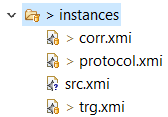
\includegraphics[scale=0.85 ]{pictures/instances.png}
    \caption{\centering{instances folder}}
    \label{setDefaultNumber}
\end{figure}

\textbf{Model generation via MODELGEN:}

The \textsf{MODELGEN\_APP} generates a consistent triple according to our rule sets without any preexisting models. It generates a hospital model, an administration target model, and the correspondence model for the connections between our source and target model.\newline

By opening the \textsf{src.xmi} you can take a look a the final model instance. You should see patients waiting in the reception or being assigned to their rooms as well as the staff members within their departments. Nurses for example which should be covering a room with patients. Look at the \textsf{trg.xmi} and you will notice that we have the same patients and staff members in this model instance. But here we focus on the shifts of the latter and treatments we assigned to their patients.

A model generator might also be helpful for testing purposes, especially scalability testing that requires large models. \newline

\textbf{Other running options:}

Let us explore the other run options as well. Although we are mainly interested in the synchronization function for our current example. It might be useful to take a step back and start with the forward and backward transformations as special cases of the general task of consistency management.\newline

\textbf{INITIAL\_FWD:}

This application requires a source model and can create or restore the target model instance in case it is given the correspondences. You might try it by deleting the \textsf{trg.xmi} in your instances folder and running the app.\newline

\textbf{INITIAL\_BWD:}

This works in the same way but requires the target side. Hence, the names \textsf{"fwd"} for forward synchronization and \textsf{"bwd"} for backward.\newline

\textbf{CC:}

Another option is the \textsf{CC\_App} which stands for consistency checking. It is used to compare the given source and target model instances by creating a respective correspondence model. \newline

\textbf{CO:}

If you want to check a complete triple of source, correspondence, and target models for consistency you can use the \textsf{CO\_App} which stands for check only. \newline

\clearpage

\textbf{Model synchronization via SYNC:}

Throughout the rest of this tutorial, we will be concentrating on model transformation via the \textbf{SYNC} operation. 

There are two reasons why initial forward and backward transformations are limited: First, they are not incremental and might incur loss of information if your bidirectional transformation is not bijective. Since both forward and backward transformation only translates the given side into a new model instance for the missing side. This can happen if one of the graphs doesn't have any correspondence for a specific node type on the other side, shifts for example.\newline

One possible solution would be to add such properties manually to the respective metamodels, but it should be clear that this defeats the purpose of having multiple metamodels for different domains or applications. The \textbf{SYNC} operation can deal with this problem because it is updating an existing output model \textbf{incrementally}. We are only adding what is necessary, missing or has changed. In this manner, unrelated parts of the model can be retained.\newline

Another reason to use \textbf{SYNC} is the improved performance. Since it works \textbf{incrementally}, the time required for an update of the current model triplet does not depend on its current size, but rather on the size of the update itself. 

Please note that you can only update either source or target model during one synchronization operation.If you changed the information on both sides of your model and want to propagate them to the respective side you should use the \textbf{integrate} operation via the \textsf{INTEGRATE\_APP} application. 

The \textbf{SYNC} operation is of course the best way to handle small updates when you are working on your eMoflon project. And henceforth we recommend using this option.\newline

\textbf{Pattern matcher configuration:}

Now let us take a closer look at these apps because there are some options to configure them.
The first line of interest is the definition of the registration helper in very application:\newline

20\hspace{0.5cm} \textcolor{Purple}{public static} IRegistrationHelper \textcolor{Blue}{\textit{registrationHelper}} = \textcolor{Purple}{new} HiPERegistrationHelper();\newline

As you can see in the package \textsf{hospital2administration.config} shown in the chart below you have the choice between the different registration helpers:\newline

\begin{figure}[h]
    \centering
    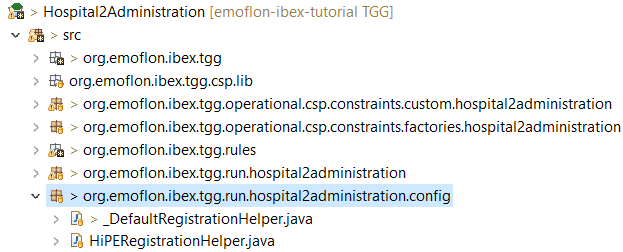
\includegraphics[scale=0.65 ]{pictures/registrationHelpers.png}
    \caption{\centering{Available registration helpers}}
    \label{setDefaultNumber}
\end{figure}

By default, a newly created project has the \textsf{\_DefaultRegistration} helper selected, but we recommend using the \textsf{HiPERegistrationHelper} for every application. \textbf{Exceptions} are the \textbf{BWD\_OPT} and the \textbf{FWD\_OPT} applications since both require the \textsf{DemoclesRegistrationHelper}.

The main difference between those two is the utilization of \textbf{different pattern matchers} which we have explained at the very beginning of our tutorial. 

\clearpage

\textbf{Saving and loading models:}

Let's look at further options within the applications:

\begin{figure}[h]
    \centering
    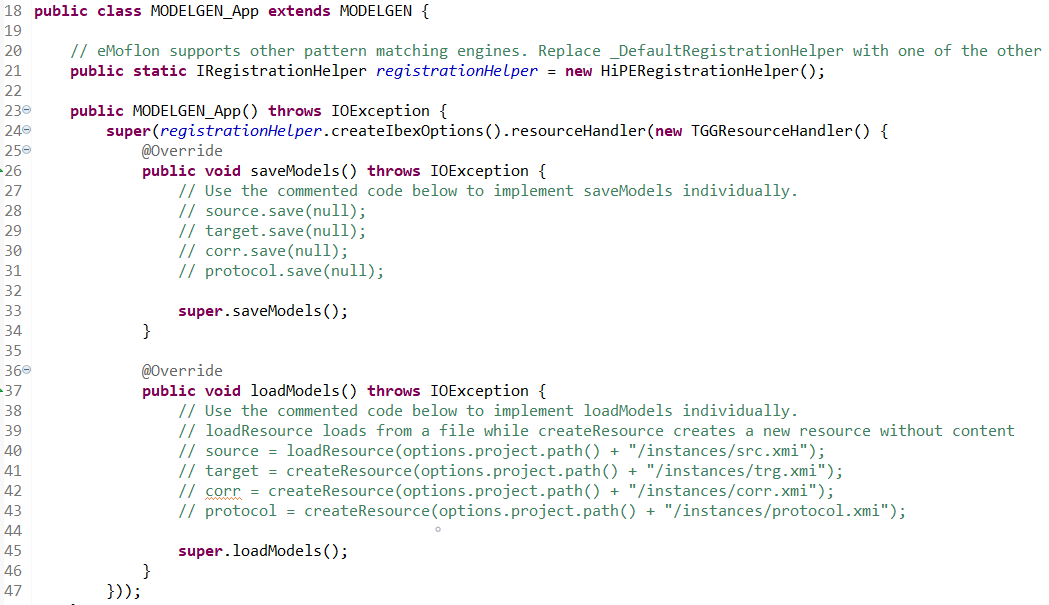
\includegraphics[scale=0.65 ]{pictures/application_MODELGEN.png}
    \caption{\centering{Example for loadModels() and saveModels() methods in the MODELGEN\_APP}}
    \label{setDefaultNumber}
\end{figure}

Depending on the operation you want to perform you can use the code which is commented out right now.\newline

\textbf{saveModels():}

This method is used to save specific components or the whole graph triplet. \textcolor{Purple}{super}.saveModels() saves all four files you can see in the instances folder. You can swap this out for one or multiple of the file specific save commands and insert a specific path for saving.\newline

\textbf{loadModels():}

This method is used to load specific components or a complete graph triplet.
For the individual load methods, we would load a model from the given path and create the corresponding resources.\newline

\textbf{Example:}

Let us walk through this exemplarily by modifying the \textsf{SYNC\_APP} to load the \textsf{hospital.xmi} we have created in the first part of this tutorial. First we want to modify the \textsf{loadModels} method to load the \textsf{hospital.xmi}.

You need to adjust the \textbf{path} to the source variable to access it. It should be saved in your workspace in the project folder of the \textsf{HospitalExample}. we will use a relative path to switch to the parent folder of our project directory then we navigate to the \textsf{hospital.xmi} which is stored in the project folder of our graph transformation project:\newline

39\hspace{0.5cm}\textcolor{Blue}{source} = loadResource(\textcolor{Blue}{options.project}.path() "\textcolor{Blue}{../HopsitalTransformationRules/hospital.xmi}");\newline

\clearpage

Since we want to synchronize our triple from the given source model, we have to create the other resources by using the \textsf{createResource} command which is commented out right now. Please remove the slash symbols for the following lines shown below:\newline

{\setstretch{1.2}

40\hspace{0.5cm}\textcolor{Blue}{target} = createResource(\textcolor{Blue}{options.project}.path() + "\textcolor{Blue}{/instances/trg.xmi}");

41\hspace{0.5cm}\textcolor{Blue}{corr} = createResource(\textcolor{Blue}{options.project}.path() + "\textcolor{Blue}{/instances/corr.xmi}");

42\hspace{0.5cm}\textcolor{Blue}{protocol} = createResource(\textcolor{Blue}{options.project}.path() + "\textcolor{Blue}{/instances/protocol.xmi}");\newline

}

After creating these resources, we still need to save them somewhere. Just uncomment the following lines in the \textsf{saveModels} method:\newline

{\setstretch{1.2}

40\hspace{0.5cm}\textcolor{Blue}{target}.save(\textcolor{Purple}{null});

41\hspace{0.5cm}\textcolor{Blue}{corr}.save(\textcolor{Purple}{null});

42\hspace{0.5cm}\textcolor{Blue}{protocol}.save(\textcolor{Purple}{null}); \newline

}

After you have saved your file and \textbf{ran} the \textbf{SYNC} application, look at the new instances. They should look different. If they are still the same, try deleting the files in the instances folder and rerun the App.

Now open up the \textsf{trg.xmi} and inspect it. The number of patients and staff members is much smaller now, but why?

In this case, we have loaded the \textsf{hospital.xmi} from our graph transformation project and in this model instance we have created the elements such as patients and staff members manually and the SYNC\_APP has generated our triple consisting of source, target, and correspondences according to the rules we defined in the TGG project. 

On the contrary, the MODELGEN\_APP created our consistent triple according to our TGG ruleset as well but \textbf{none of the values were bound} and hence the triple was created with random values as we defined it in the attribute conditions. Additionally, it would have done it \textbf{infinitely} if we had not defined the criteria to stop the execution of the application.\newline

You can find these criteria in the main method of the applications. For example, we set a stop criterion based on the runtime:\newline

\textcolor{Tan}{stop}.setTimeOutInMS(1000);\newline

For this example, we terminate our application after approximately \textsf{1000 ms}with the keyword \textcolor{Tan}{stop}. By using the auto-completion function you can see the other options you can set as \textbf{stop criteria}.

For example, if we want to execute a rule a certain number of times we can type:\newline

\textcolor{Tan}{stop}.setMaxRuleCount("HospitaltoAdministrationRule", 1); \newline

In this case, we limited the number of applications of the HospitalToAdministration to 1. You can find a list of possible stop criteria in the \textbf{appendix} below.

\clearpage

\subsection{ Debugging in TGGs}

A note on the debugging app you can find in the \textsf{.debug} package shown below:\newline

\begin{figure}[h]
    \centering
    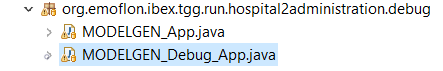
\includegraphics[scale=0.65 ]{pictures/debugPackage.png}
    \caption{\centering{\textsf{.debug} package}}
    \label{setDefaultNumber}
\end{figure}

There is no need for this when your set of triples is created without any errors. But when the rules or correspondences are not working in the way you want them to work you can run the generation in debug mode.

Once you run the \textsf{MODELGEN\_Debug\_App.java} a new window like the one in chart below pops up. On the top left, you can see the rules which have already been applied, the other rules are crossed out. On the right, you can see the respective visualization, and on the bottom left you can see the order in which the rules were applied. \newline

If you hit the \textbf{apply} button on the left now you will apply the next rule according to the way, we have defined it in the java files. This works like debugging in Java and leads you step by step through the application of our ruleset and updates of the visualization.

\begin{figure}[h]
    \centering
    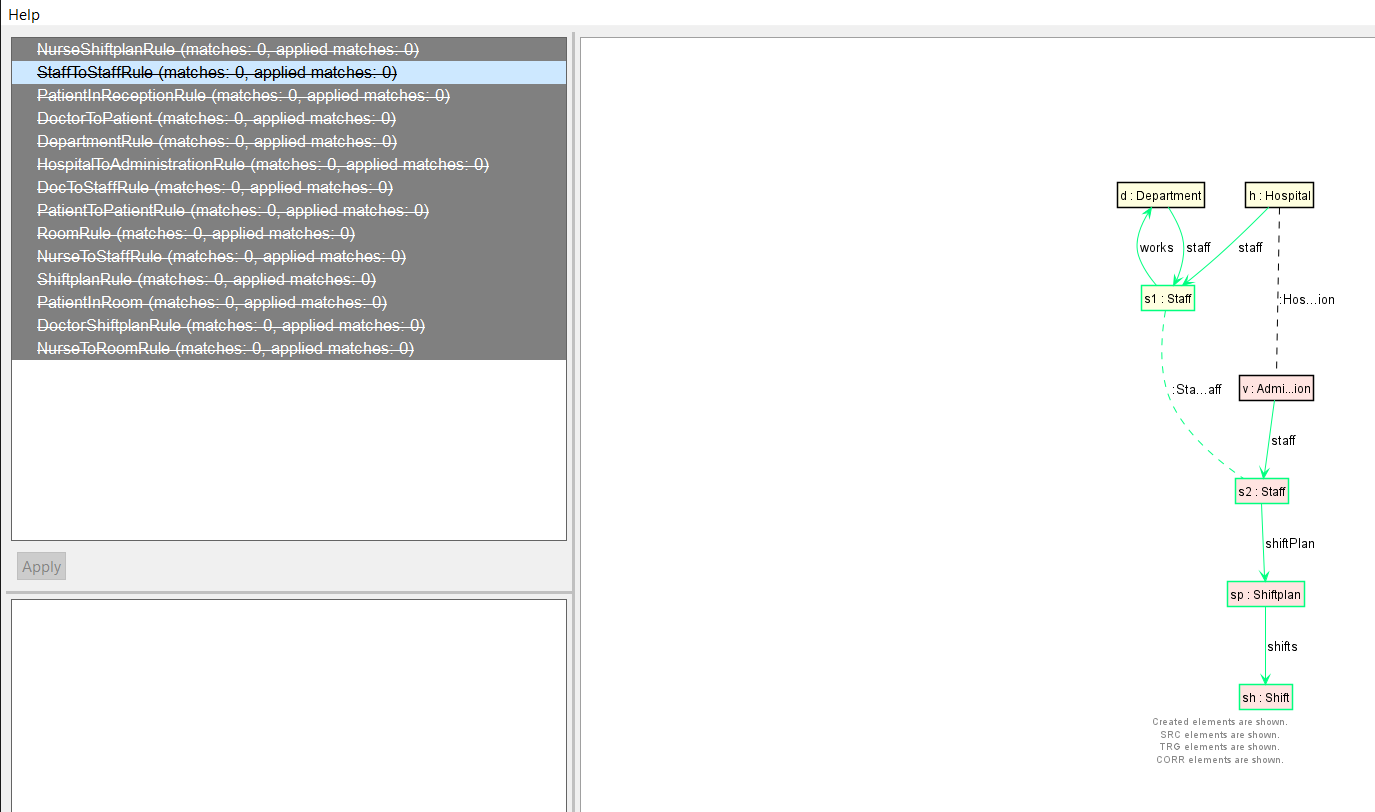
\includegraphics[scale=0.4 ]{pictures/debugWindow.png}
    \caption{\centering{Debugging window}}
    \label{setDefaultNumber}
\end{figure}


\clearpage